\documentclass[a4paper]{article}
\usepackage[utf8]{inputenc}
\usepackage[czech]{babel}
\usepackage[margin=13mm, tmargin=15mm, bmargin=12mm]{geometry}
\usepackage{multirow}
\usepackage{tikz}
\usetikzlibrary{calc}
\usepackage{chngpage}
\usepackage{tabularx}
\usepackage{fancyhdr}
\usepackage{mathptmx}
\usepackage{lipsum}
\usepackage{float}
\usepackage{longtable}

\renewcommand{\baselinestretch}{1.15}
\pagenumbering{gobble}
\pagestyle{fancy}
\renewcommand{\headrulewidth}{0pt}

\newcommand{\jmeno}{David Škrob, Tom\'{a}\v{s} N\'{a}zler, Vojta Nevrlý}
\newcommand{\trida}{L3A}
\newcommand{\poradovecislo}{}
\newcommand{\nazevulohy}{Číslicové obvody}
\newcommand{\cisloulohy}{}
\newcommand{\predmet}{Technické měření}
\newcommand{\skupina}{}
\newcommand{\datummereni}{4.5.2022}
\newcommand{\datumodevzdani}{1.6.2022}
\newcommand{\klasifikace}{}
\begin{document}
\fancyhead{
\begin{tikzpicture} [overlay,remember picture]
       \draw
        ($ (current page.north west) + (1cm, -12mm) $)
        rectangle
        ($ (current page.south east) + (-1cm,12mm) $);
\end{tikzpicture}
}

\renewcommand{\arraystretch}{2}
\shorthandoff{-}

{
\begin{adjustwidth}[]{-3mm}{-3mm}
\centering
\vspace*{-7mm}
\begin{tabularx}{\linewidth}{l|X|p{3cm}}
\multirow{2}{25mm}{\centering SPŠ a VOŠ technická Brno, Sokolská 1} &
\textbf{LABORATORNÍ CVIČENÍ Z ELEKTROTECHNIKY} & Třída: \trida \\
\cline{2-3}
 & Jméno a příjmení: \jmeno & Poř. Číslo: \poradovecislo \\
\hline
\end{tabularx}

\begin{tabularx}{\linewidth}{X|p{3cm}}
Název úlohy: \nazevulohy & Číslo úlohy: \cisloulohy \\
\hline
Zkoušený předmět: \predmet & Skupina: \skupina \\
\hline
\end{tabularx}

\begin{tabularx}{\linewidth}{X|X|X}
Datum měření: \datummereni &  Datum odevzdání: \datumodevzdani &  Klasifikace: \klasifikace \\
\hline
\end{tabularx}

\end{adjustwidth}
}

\shorthandon{-}

\section*{Zadání}
1) Ověřte funkci jednotlivých obvodů. Zjistěte, zda obvody 7472 a následující jsou řízeny stavem, náběžnou nebo sestupnou hranou jednotlivých vstupů. U obvodu 7472 a následujících znak \& znamená, že pokud vstup není připojen, je vnitřně nastaven na logickou~1.\begin{itemize}
	\item 7400 – 4x logický člen NAND
	\item  7402 – 4x logický člen NOR
	\item 7404 – 6x logický člen NOT
	\item 7408 – 4x logický člen AND
	\item 7432 – 4x logický člen OR
	\item 7472 – klopný obvod JK včetně vstupů S, R
	\item 7474 – 2x klopný obvod D včetně vstupů S, R (lze použít i jako klopný obvod RS)
	\item 7493 – čtyřbitový čítač (s nulováním) včetně vstupu R, ve skutečnosti je o dva čítače, jednobitový na vstupu A a tříbitový na vstupu BD - jak obvod zapojíte, aby fungoval jako čtyřbitový čítač? Jak se obvod chová při přetečení?
	\item 74164 – posuvný registr (s nulováním)
\end{itemize}
2) Realizujte základní logické funkce (NOT, AND, OR, NOR, XOR – pouze ověření) pomocí hradel NAND. Kdo stíhá může totéž zkusit i pro hradla NOR – samostatná práce.
Schémata těchto zapojení pomocí hradel NAND budou součást protokolu. 
\section*{Teorie}
\begin{figure}[h!]
	\renewcommand\figurename{Obvod}
	\centering
	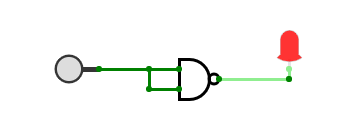
\includegraphics[width=0.6\linewidth]{not.png}
	\caption{Logicky obvod  NOT za pomocí logických obvodů NAND}
	\label{fig:not}
\end{figure}
\begin{figure}[h!]
	\renewcommand\figurename{Obvod}
	\centering
	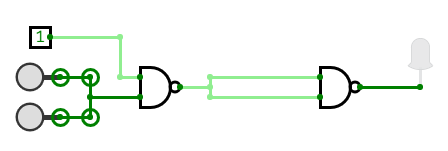
\includegraphics[width=0.6\linewidth]{or.png}
	\caption{Logicky obvod  OR za pomocí logických obvodů NAND}
	\label{fig:or}
\end{figure}
\begin{figure}[h!]
	\renewcommand\figurename{Obvod}
	\centering
	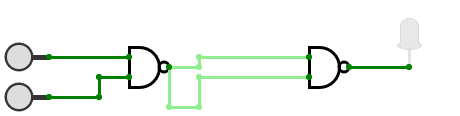
\includegraphics[width=0.6\linewidth]{and.png}
	\caption{Logicky obvod AND za pomocí logických obvodů NAND}
	\label{fig:and}
\end{figure}
\begin{figure}[h!]
	\renewcommand\figurename{Obvod}
	\centering
	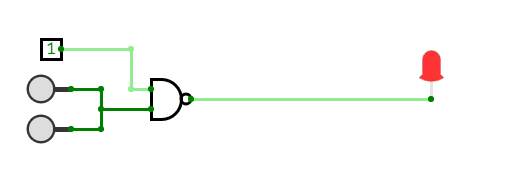
\includegraphics[width=0.6\linewidth]{nor.png}
	\caption{Logicky obvod NOR za pomocí logických obvodů Nnor}
	\label{fig:nor}
\end{figure}
\begin{figure}[h!]
	\renewcommand\figurename{Obvod}
	\centering
	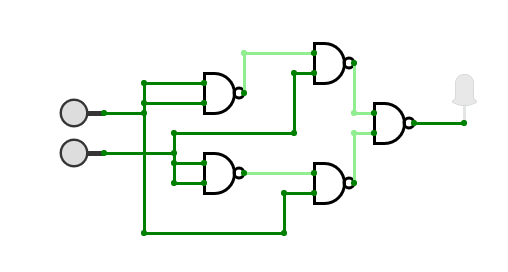
\includegraphics[width=0.6\linewidth]{xor.png}
	\caption{Logicky obvod XOR za pomocí logických obvodů Nxor}
	\label{fig:xor}
\end{figure}
\newpage
\section*{Vypracování}
\begin{itemize}
\item [7400] nand - funguje
\item [7402] nor - funguje
\item [7404] not - funguhe
\item [7408] and - funguje
\item [7432] or - funguje
\item [7474] - poslaní na vzestupné hraně poslání pomocí clocku a data jsou vstupy, set a reset mají větší prioritu než data a clock
\item [7493] - sčítání funguje na sestupné hraně.
\item [74164] - cr nesmí být zapojen, a když obě hodnoty v registru jsou 1 jinak nula cl posouvá řadu.
\item [7472] - funguje tak jak očekáváno
\end{itemize}
\section*{Závěr}
První část, byla díky naší neznalosti obvodů typu R, S byla obtížná, avšak díky tomu již víme jak obvody typu R a S fungují. Díky našemu zájmu o logická hradla, byla druhá část protokolu jednoduchá, takže mělo pro nás měření ideální obtížnost.
\section*{Použité pomucky:}
\begin{tabularx}{\linewidth}{c|c|c|c}
	Přístroj – pomůcka & Typ & Rozsah (pouze analogové)
	& Poznámka \\
	\hline
	RC&2000&&\\
\end{tabularx}
\end{document}